\chapter{Grafos Estáticos e Dinâmicos} \label{grafoestdin}
Segundo \cite{negreirosbook}, um grafo é formado por três conjuntos:\\
- Vértice ou Nodos: representam os pontos (N ou V);\\
- Arestas ou Elos: representam ligações não orientadas entre os Nodos (E);\\
- Arcos: representam ligações orientadas entre os vértices (A).\\
O Grafo pode ser representado da seguinte forma: $G(V, E, A)$.

Grafo orientado ou assimétrico - $G(V, A)$, $E = \emptyset$: uma aresta $(u,v)$ é dita orientada de $u$
para $v$ se o par $(u,v)$ for ordenado, com $u$ precedendo $v$.

Numa abordagem computacional, um programa orientado a objetos pode ser associado a um grafo cujos vértices
representam as classes definidas no programa, e cujas arestas indicam a herança entre as classes.
Existe uma aresta de um vértice $v$ a um vértice $u$ se a classe para $v$ estender a classe de $u$.
Logo o grafo é assimétrico, pois essas arestas são dirigidas ou orientadas porque a relação de herança
só existe em uma direção. Outro exemplo segue na figura \ref{fig:assimetrico}.

\begin{figure}[htbp]
\centering
 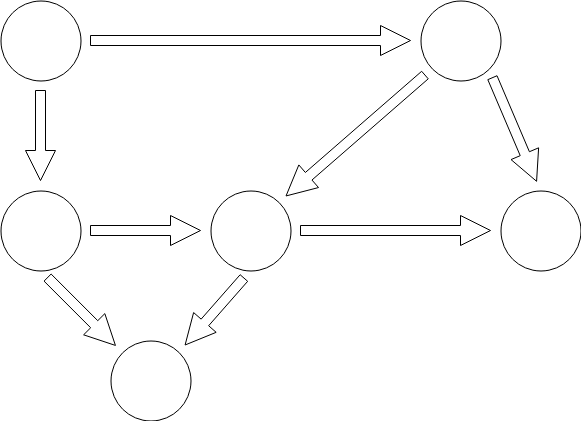
\includegraphics[width=.55\textwidth]{chapters/fig/assimetrico1.png}
\caption{Grafo Orientado ou Assimétrico}
\label{fig:assimetrico}
\end{figure}

Grafo não orientado ou simétrico - $G(V, E)$, $A = \emptyset$: uma aresta $(u,v)$ é dita não-orientada
se o par $(u,v)$ não for ordenado. As aresta não-orientadas são por vezes denotadas como conjunto ${u,v}$,
mas, para simplificar, é utilizado a notação de pares ordenados $(u,v)$, notando que no caso não-orientados
$(u,v)$ é o mesmo que $(v,u)$ \cite{goodrich}, figura \ref{fig:simetrico}.

Também é possível visualizar colaborações entre pesquisadores de certa área construindo um grafo cujos vértices são
associados aos pesquisadores e cujas arestas conectam pares de vértices associados aos pesquisadores
que escreveram juntos um artigo ou livro (Figura \ref{fig:goodrich}). Tais arestas são não-orientadas porque
a co-autoria é uma relação simétrica, ou seja, se A é co-autor de B, então necessariamente B é co-autor de A.

\begin{figure}[htbp]
\centering
 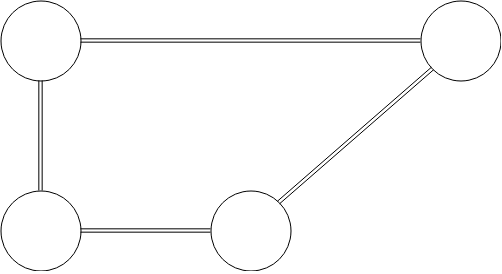
\includegraphics[width=.55\textwidth]{chapters/fig/simetrico1.png}
\caption{Grafo não Orientado ou Simétrico - $G(V,E)$}
\label{fig:simetrico}
\end{figure}

\begin{figure}[htbp]
\centering
 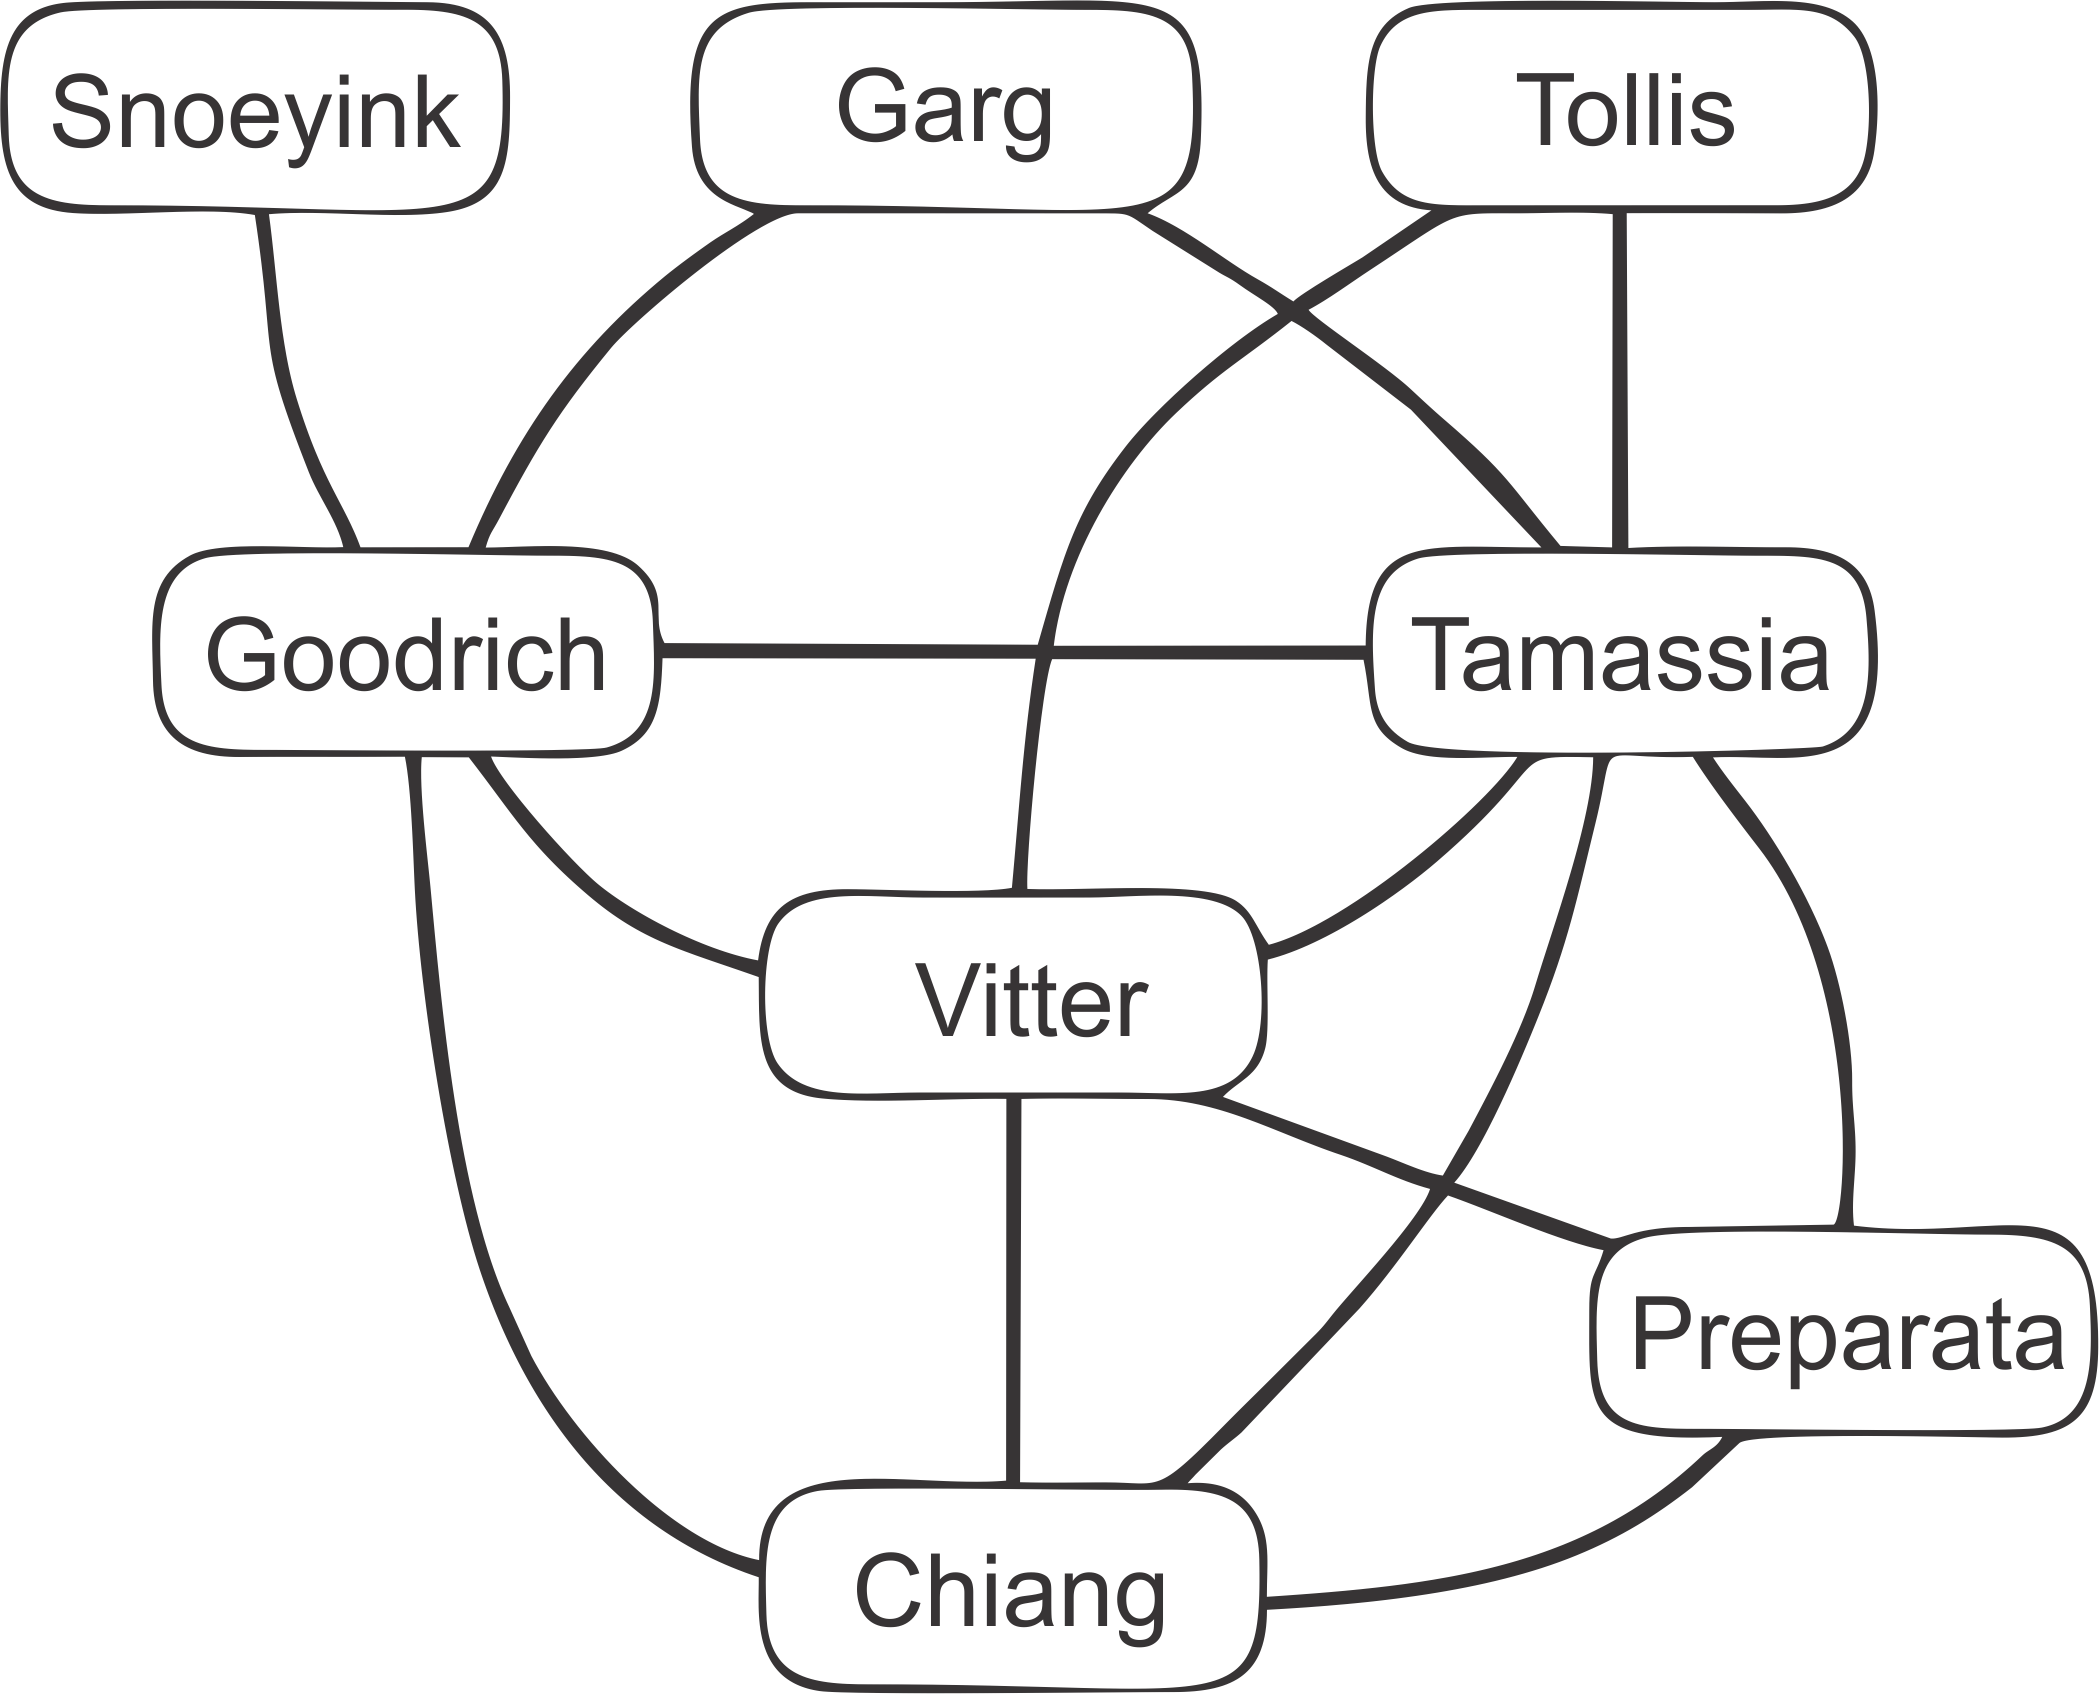
\includegraphics[width=.55\textwidth]{chapters/fig/goodrich.png}
\caption{Grafo de co-autoria de alguns autores}
Fonte: Elaboração própria, baseada em \cite{goodrich}
\label{fig:goodrich}
\end{figure}


\pagebreak

\cite{goodrich} diz que se todas as arestas em um grafo forem não-dirigidas,
então diz-se que o grafo é um grafo não-dirigido. De forma similar, um grafo dirigido, ou dígrafo, é um grafo em
que todas as arestas são dirigidas. Um grafo que tem arestas dirigidas e não-dirigidas é chamado de grafo misto, 
como mostra a figura \ref{fig:misto}.
Um mapa viário de uma cidade pode ser modelado como um grafo cujos vértices são cruzamentos ou finais de ruas, e cujas arestas
podem ser trechos de ruas sem cruzamentos. Este grafo tem arestas não-dirigidas, representando ruas de dois sentidos,
e arestas dirigidas, correspondendo a trechos de um único sentido. Assim, um grafo representando as ruas de uma cidade
é um grafo misto.

\begin{figure}[htbp]
\centering
 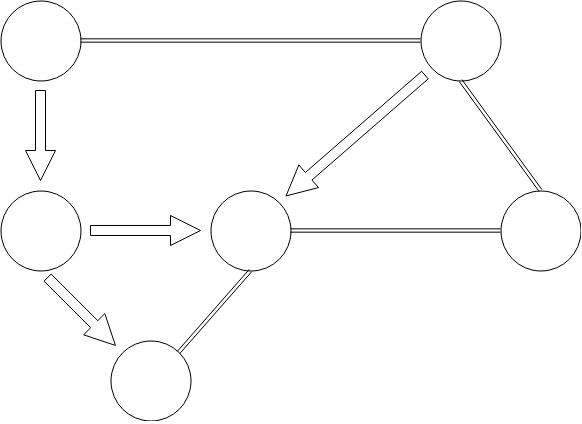
\includegraphics[width=.55\textwidth]{chapters/fig/misto1.png}
\caption{Grafo Misto - $G(V,E,A)$}
\label{fig:misto}
\end{figure}

\section{Rede de Topologia Estática}
Várias estruturas representam esse tipo de rede, como: estrutura matricial,
estrutura de listas encadeadas, estrutura de listas duplamente
encadeadas, dentre outras \cite{negreiros}.
Segundo \cite{cormen}, existem duas maneiras para representar um grafo $G = (V,E)$:
como uma coleção de listas de adjacências ou como uma matriz de adjacências. A representação
de lista de adjacências em geral é preferida, porque ela fornece um modo compacto para representar grafos esparsos,
onde para os quais $|E|$ é muito menor que $|V|^2$. Contudo, uma representação de matriz de adjacências pode ser
preferível, quando o grafo é denso, onde $|E|$ está próximo de $|V|^2$, ou quando é preciso ter a possibilidade
de saber com rapidez se existe uma aresta conectando dois vértices dados.

Segundo \cite{goodrich}, uma Estrutura Matricial ou matriz de adjacência estende a estrutura de armazenamento
das arestas com um componente adicional. Com isso, aumenta-se a lista de arestas com uma matriz (um arranjo de duas dimensões) A,
que permite que se determine adjacências entre pares de vértices em tempo constante. Na matriz de adjacência,
consideramos os vértices como sendo os inteiros no conjunto \{0,1,...,n-1\}, e as arestas como sendo pares desses inteiros.
Isso permite armazenar referências para as arestas nas células de um arranjo de duas dimensões $A_{n x n}$.

Segundo \cite{goldbarg}, uma matriz $A = |a_{ij}|$ quadrada de ordem $n$ é denominada matriz de adjacência de $G = (V, E)$ quando:\\
\indent $a_{ij}$ = 1, se $\exists(i,j)$ $\in$ $E$\\
\indent $a_{ij}$ = 0 em caso contrário.

As figuras \ref{fig:matriznaodirecionada} e \ref{fig:matrizdirecionada} apresentam exemplos de matrizes de adjacências para
grafos não direcionados e direcionados, respectivamente.

\begin{figure}[htbp]
\centering
 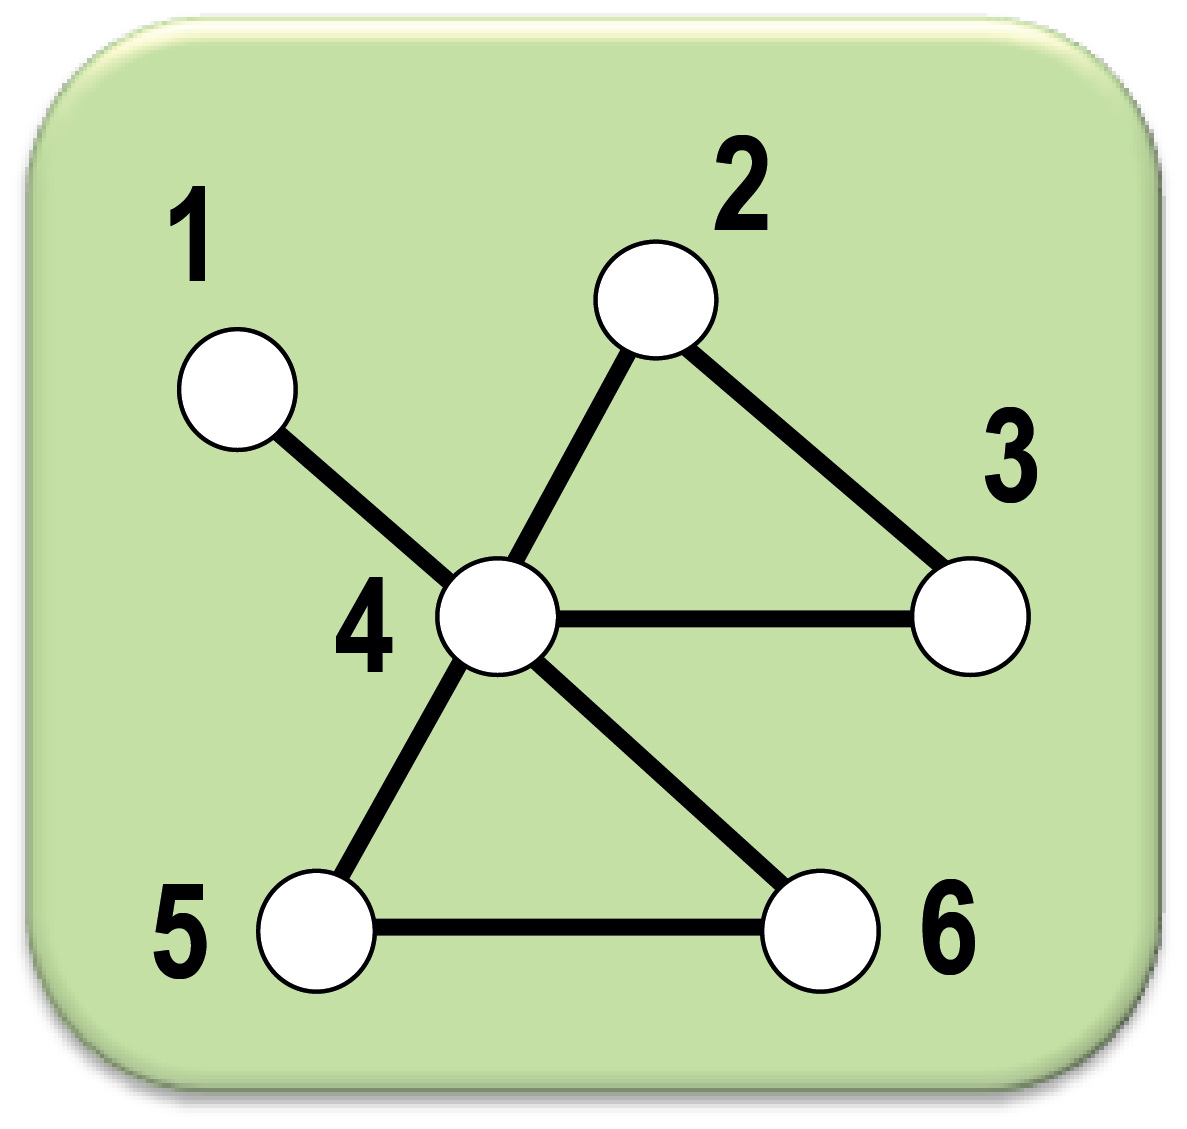
\includegraphics[width=.30\textwidth]{chapters/fig/cal_fig_091a.jpg}
 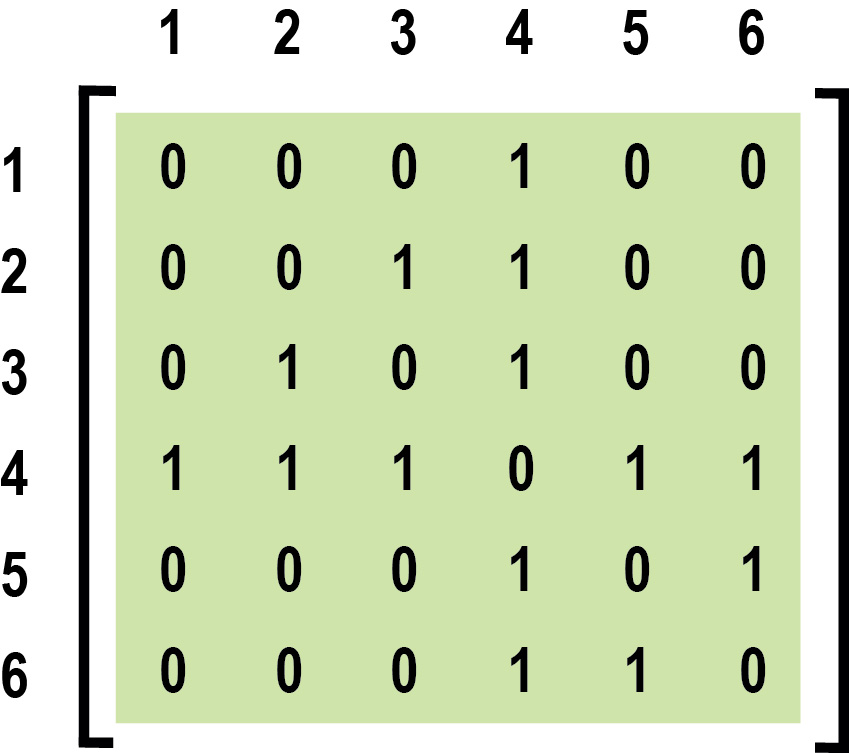
\includegraphics[width=.35\textwidth]{chapters/fig/cal_fig_091b.jpg}
\caption{Matriz de adjacências de grafo não direcionado}
Fonte: \cite{goldbarg}
\label{fig:matriznaodirecionada}
\end{figure}

\begin{figure}[htbp]
\centering
 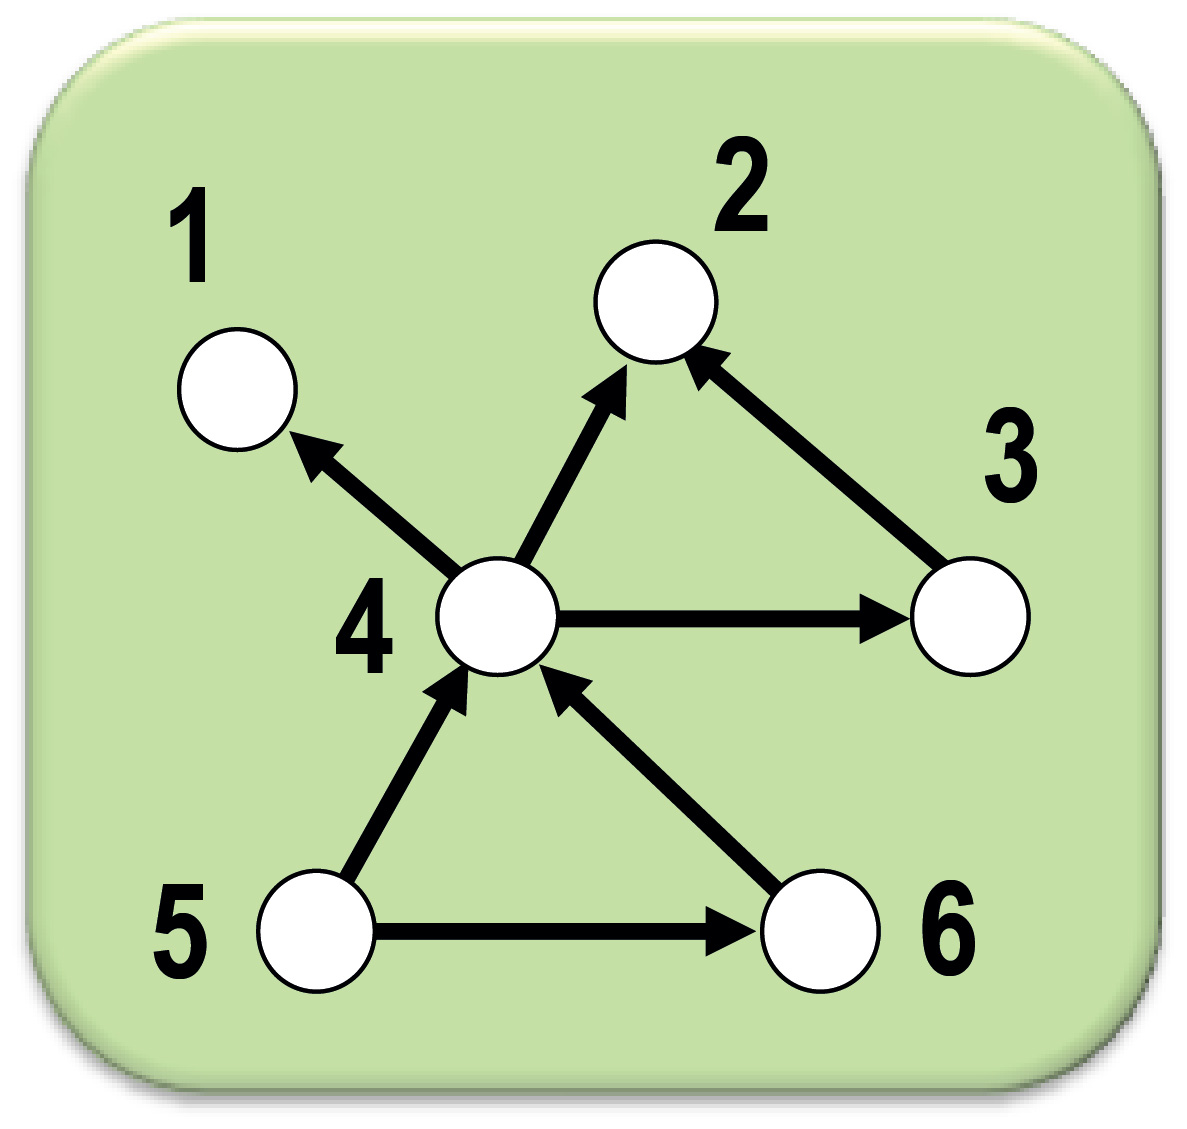
\includegraphics[width=.30\textwidth]{chapters/fig/cal_fig_092a.jpg}
 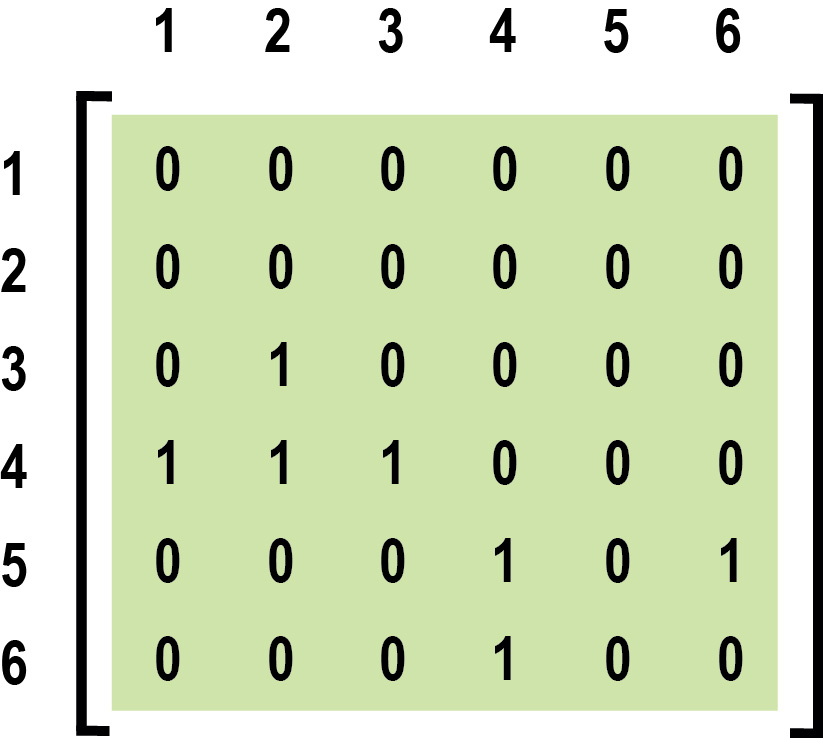
\includegraphics[width=.35\textwidth]{chapters/fig/cal_fig_092b.jpg}
\caption{Matriz de adjacência de grafo direcionado}
Fonte: \cite{goldbarg}
\label{fig:matrizdirecionada}
\end{figure}

Em Listas Encadeadas, segundo \cite{negreirosbook} e \cite{cormen}, quando se deseja armazenar um grafo pouco denso, ou seja,
$D_{max} \leqslant$ $\dfrac{|V|}{2}$ é mais vantajoso usar estruturas mais eficientes de armazenamento, assim como as listas
e vetores de listas. Neste caso, os vértices estão posicionados no vetor principal, onde a própria célula do vetor
guarda o rótulo do vértice que entrou primeiro e assim sucessivamente, como numa pilha. As pilhas, que derivam de cada
célula do vetor, podem ser construídas levando-se em conta as ligações de arcos/elos ao elemento vértice da célula
que o gera. No índice de cada célula de lista, mantém-se pelo menos uma informação contendo o vértice de ligação,
figura \ref{fig:listaencad}.
\FloatBarrier
\noindent $Type$\\
Lista: $\string^$ Lta;\\
$Lta$ = Record\\
$v$ : word; \{ Arco/elo ligado a VV\_i \}\\
$prx$ : Lista;\\
end;\\
$VV$ = Array[1..n] of Lista;\\

\begin{figure}[htbp]
\centering
 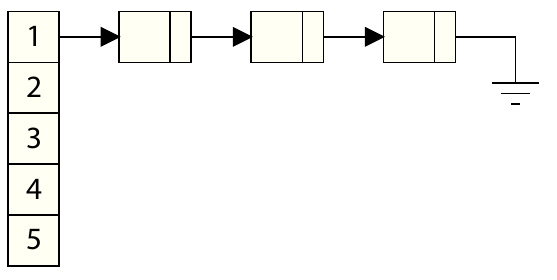
\includegraphics[width=.65\textwidth]{chapters/fig/listaencad.png}
\caption{Representação em Listas Encadeadas de um grafo}
Fonte: \cite{dynagraph} apud \cite{negreirosbook}
\label{fig:listaencad}
\end{figure}

Estruturas de Listas Duplamente Encadeadas são da forma, representada na figura \ref{fig:listdupla}, segundo \cite{negreirosbook}:
\FloatBarrier
\noindent $Type$\\
Lista: $\string^$ Lta;\\
$Lta$ = Record\\
$v$ : word; \{ Arco/elo ligado a VV\_i \}\\
$prx$ : Lista;\\
$ant$ : Lista;\\
end;\\
$VV$ = Array[1..n] of Lista;\\

\begin{figure}[htbp]
\centering
 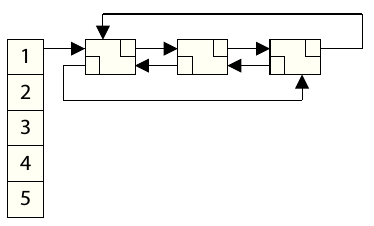
\includegraphics[width=.65\textwidth]{chapters/fig/listdupla.png}
\caption{Representação de um grafo em Listas Duplamente Encadeadas}
Fonte: \cite{dynagraph} apud \cite{negreirosbook}
\label{fig:listdupla}
\end{figure}

Esta forma tem grandes vantagens na mobilidade e acessibilidade sobre os dados de um arco.
Porém, sofre em relação à lista simples, pois usa mais memória de armazenamento com pelo
menos 4 bytes a mais por arco.

\pagebreak

\section{Redes Dinâmicas}

Em \cite{harary}, são definidas três tipos de redes: rede de nodos, rede de elos e rede ponderada.
\begin{itemize}
\item Uma rede de nodos (ou grafo de nodos ponderados) é uma tripla $(V, E, f)$, onde $V$ é um conjunto
de vértices, $E$ é um conjunto de arestas $\{u,v\}$, e $f$ é uma função, $f: V \rightarrow N$ onde $N$
é um sistema numérico, atribuição de um valor ou um peso.
\item Uma rede de elos (ou grafo de arestas ponderadas) é uma tripla $(V, E, g)$, definida de forma semelhante.
\item Uma rede Ponderada (ou grafo totalmente ponderado) tem pesos atribuídos a ambos nós e arestas.
\end{itemize}

Outro tipo de rede é chamada de rede genérica, que contém atributos e características.

Grafo Dinâmico $G^t(V^t, L^t)$ é todo grafo que modifica seus vértices ($V^t$) e/ou ligações ($L^t$)
ao longo de um período de tempo ($H \in [T_i, T_k]$). Ou seja, as entidades $V$(um conjunto de nodos),
$E$(um conjunto de elos), $f$(mapeamento de vértices para números) e $g$(mapeamento de arestas para números)
podem se modificar dentro do intervalo H.
Logo, existem cinco tipos básicos de Grafos Dinâmicos.

\begin{itemize}
\item Em um grafo ou dígrafo com nós dinâmicos, o conjunto $V$ varia com o tempo. Assim, alguns nós podem
ser adicionados ou removidos. Quando os nós são removidos, as arestas ligadas a eles também são removidas; 
\item Em um grafo ou dígrafo com elos dinâmicos, o conjunto $E$ varia com o tempo. Assim, os arcos podem
ser adicionados ou removidos a partir do grafo ou dígrafo;
\item Em um grafo dinâmico de nodos ponderados, a função $f$ varia com o tempo. Assim, os pesos nos nós também variam;
\item Em um grafo dinâmico de elos ponderados, a função $g$ varia com o tempo;
\item Em um grafo dinâmico totalmente ponderado (ou grafo com topologia e atributos dinâmicos), ambas as funções $f$ e $g$
podem variar com o tempo.
\end{itemize}

\subsection{Topologia Estática e Atributos Dinâmicos}
Nesta rede os vértices e as arestas são constantes ao longo do tempo, mas seus atributos podem ser alterados.
O grafo é definido como $G(V^t, L^t)$, onde $V^t$ e $L^t$ são constantes no horizonte $H \in [T_i, T_k]$.
A figura \ref{fig:tead} exemplifica este grafo.

\begin{figure}[htbp]
\centering
 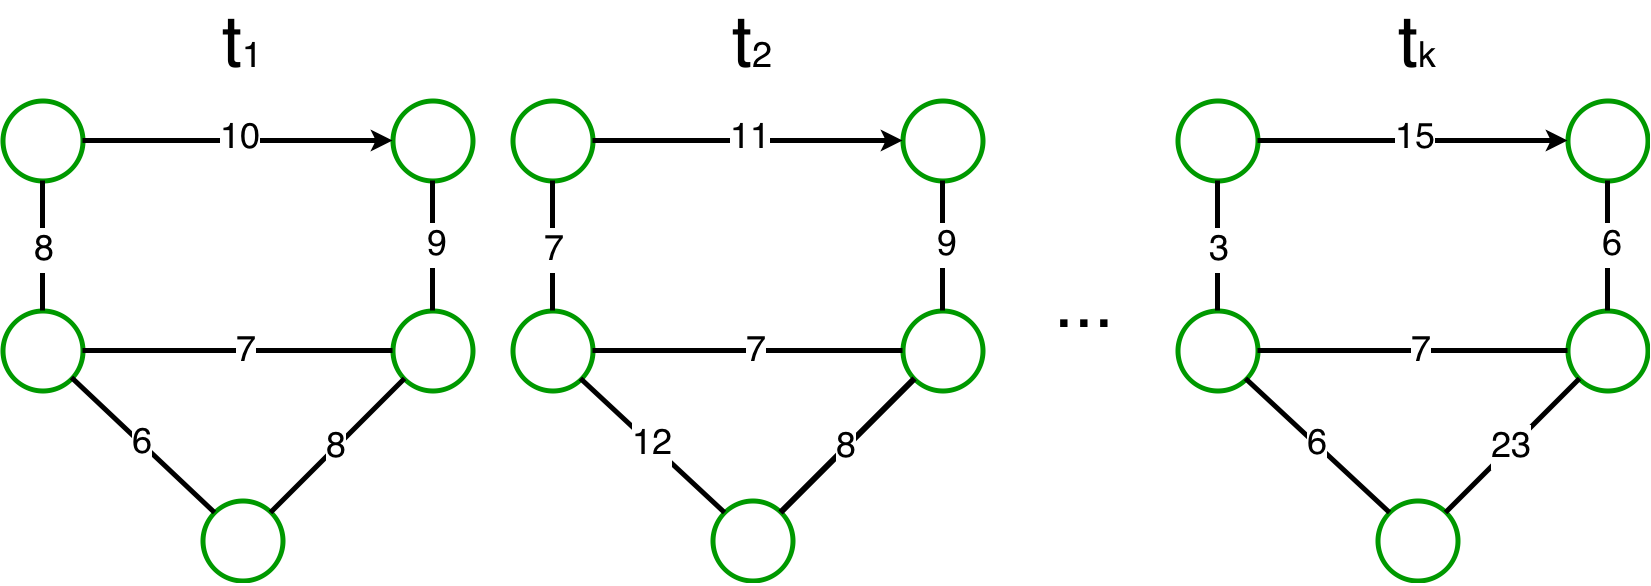
\includegraphics[width=.99\textwidth]{chapters/fig/tead.png}
\caption{Grafo com Topologia Estática e Atributos Dinâmicos}
\label{fig:tead}
\end{figure}

\subsection{Topologia Dinâmica e Atributos Estáticos}
\label{subsec:topdinatribest}
Nesta rede, ao longo do tempo, os vértices e as arestas podem ser removidos, adicionados e até mesmo
modificados para outra posição, mas suas características como espessura, cor e tamanho são fixas.
O grafo é definido como $G(V^t, L^t)$, onde $V^t$ e $L^t$ mudam no horizonte $H \in [T_i, T_k]$,
porém os atributos sempre serão os mesmos. A figura \ref{fig:tdae} mostra um exemplo desse grafo.

\begin{figure}[htbp]
\centering
 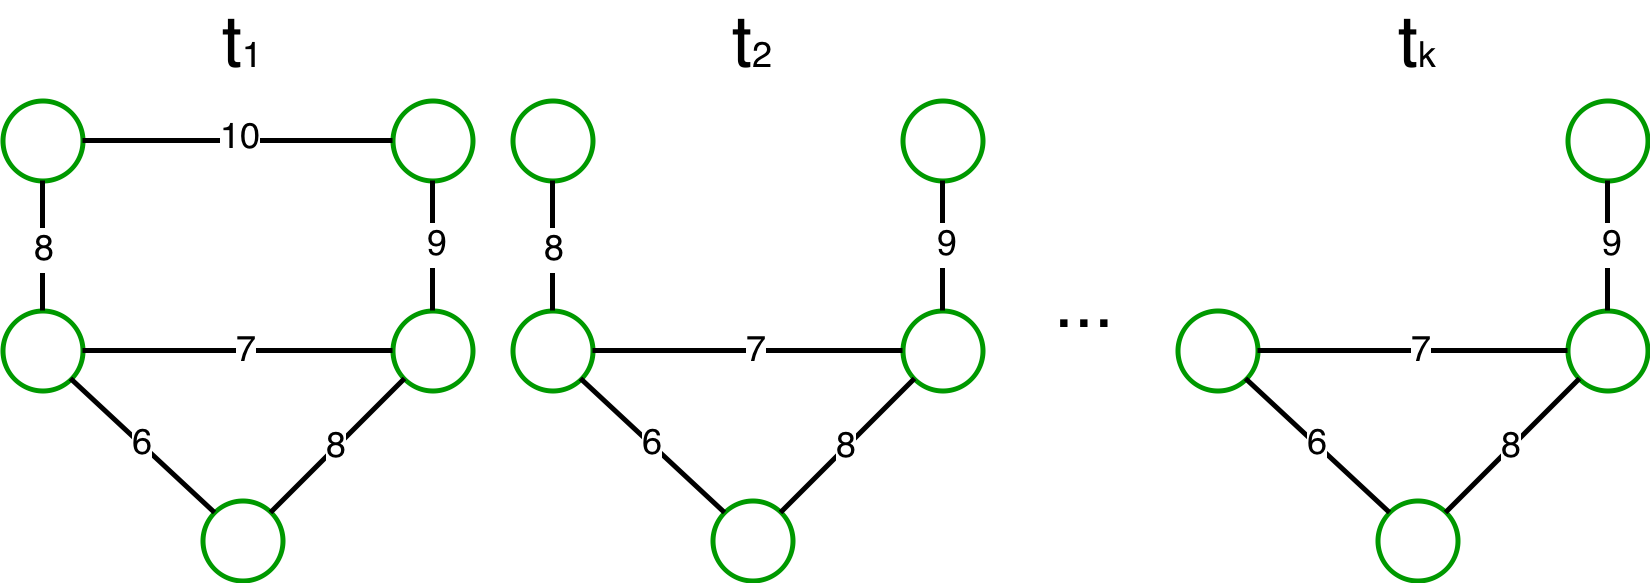
\includegraphics[width=.99\textwidth]{chapters/fig/tdae.png}
\caption{Grafo com Topologia Dinâmica e Atributos Estáticos}
\label{fig:tdae}
\end{figure}

\FloatBarrier

\subsection{Topologia e Atributos Dinâmicos}
\label{subsec:topdinatridin}
Nesta rede, o grafo é definido como $G(V^t, L^t)$, onde $V^t$ e $L^t$ mudam no horizonte $H \in [T_i, T_k]$, como
visto na figura \ref{fig:tdat}
Estas redes são mais complexas \cite{dynagraph}, pois lidam com grande volume de dados comparadas as redes anteriores descritas.

\begin{figure}[htbp]
\centering
 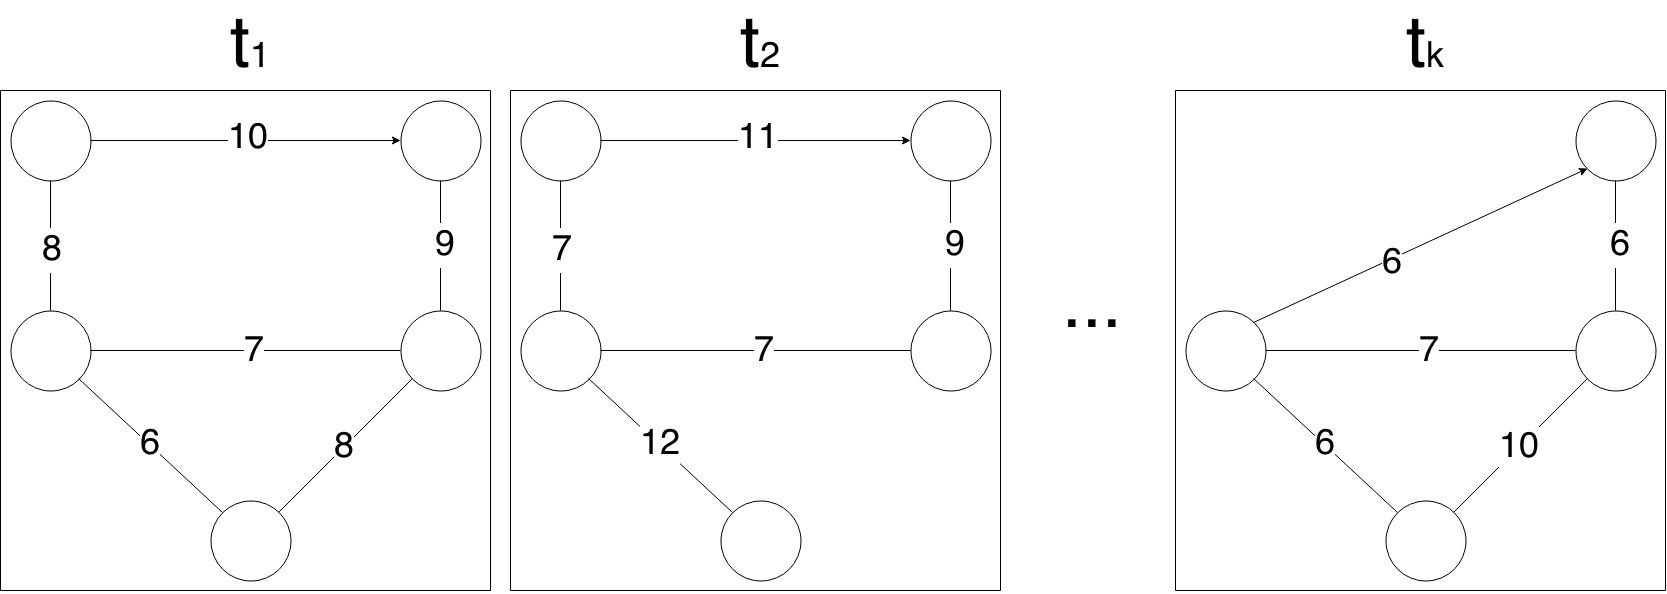
\includegraphics[width=.99\textwidth]{chapters/fig/tdat.png}
\caption{Grafo com Topologia e Atributos Dinâmicos}
\label{fig:tdat}
\end{figure}

\FloatBarrier

\section{Geração e manutenção de Redes Dinâmicas}
Os seguintes trabalhos abordam grafos dinâmicos e são utilizados como base deste trabalho:
\begin{itemize}
\item Modelo de Kim e Anderson, \cite{kim}
\item Gephi, \cite{gephi}
\item Dynagraph, \cite{dynagraph}
\end{itemize}


\subsection{O modelo de Kim e Anderson}
A ideia central de \cite{kim} é modelar uma rede dinâmica como digrafos orientados
ao tempo (time-ordered graph), que é gerada através da ligação de instantes temporais com arestas
direcionadas que unem cada nó ao seu sucessor no tempo. Com isso, transformar uma rede dinâmica
em um grafo maior, mas facilmente analisável. Isto permite não só a utilização dos algoritmos
desenvolvidos para gráficos estáticos, mas também para melhor definir métricas para
gráficos dinâmicos. Os recursos incluídos permitem que se faça avaliações das métricas
de centralidade relacionadas ao grau, proximidade e intermediação, de uma forma
natural para o caso dinâmico.

Segundo \cite{kim} um sistema de grafos dinâmicos é um objeto de representação visual que pode descrever
melhor o comportamento dinâmico de objetos relacionados a eventos dinâmicos e introduzir
novas formas de enxergar ou descrever a evolução de eventos dinâmicos na natureza.

\cite{kim} trata um modelo de redes dinâmicas, com a seguinte definição: Assumindo que a duração
de um período observado é finito, de um tempo inicial $t_{start}$ até o tempo final $t_{end}$. Sem perda de
generalidade, é dado $t_{start}$ = $0$ e $t_{end}$ = $T$. Uma rede dinâmica $G^D_{0,T}$ = $(V, E_{0,T})$ consiste
em um conjunto de vértices e arestas temporais existentes no intervalo de tempo $[0,T]$, onde
os vértices $V$ e conjunto de arestas temporais $E_{0,T}$, onde uma aresta $(u,v)_{i,j}$ $\in$ $E_{0,T}$
existe entre vértices $u$ e $v$ em um intervalo de tempo $[i,j]$, tal que $i \leqslant T$ e $j \geqslant 0$.

Neste modelo, em uma rede dinâmica, o conjunto de vértices $V$ é sempre o mesmo, enquanto o conjunto de arestas existentes
mudam ao longo do tempo.

Para representar a duração de cada $snapshot$ (ou janela de tempo) a letra $w$ é utilizada para especificar, $T$/$n$,
expresso em alguma unidade de tempo (como segundos ou horas).

Conforme \cite{kim}, uma rede dinâmica pode ser representada como uma série de grafos estáticos
$G_1, G_2, ..., G_N$. A notação $G_t(1 \leqslant t \leqslant n)$ representa o grafo agregado que consiste
de um conjunto de vértices $V$ e um conjunto de arestas $E_t$ onde uma aresta $(u,v)$ $\in$ $E_t$ existe
somente se uma aresta temporal $(u,v)_{i,j}$ $\in$ $E_{0,T}$ existe entre os vértices $v$ e $u$ no intervalo
de tempo $[i,j]$ tal que $i \leqslant wt$ e $j > w(t-1)$. $G_t$ é o t-ésimo $snapshot$ temporal de uma
rede dinâmica $G^D_{0,T}$ durante a t-ésima janela de tempo.

\begin{table}[htbp]
	\centering
	\begin{tabular}{l l l l l l}
	\toprule
	\\Aresta & & & & & Intervalo de tempo\\
	\midrule
	\\(A,C) & & & & & [1,1]\\
	\\(A,D) & & & & & [2,2]\\
	\\(B,D) & & & & & [2,3]\\
	\\(C,D) & & & & & [3,3]\\
	\bottomrule
	\end{tabular}
\caption{Exemplo de contatos (arestas) em uma rede dinâmica}
 \label{tab:kim}
\end{table}

\begin{figure}[htbp]
\centering
 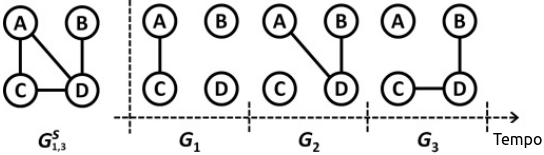
\includegraphics[width=.65\textwidth]{chapters/fig/kim.png}
\caption{Comparação entre a representação de grafos agregados(esquerda) e representação de sequência temporal(direita)}
Fonte: \cite{kim}
\label{fig:grafoKim}
\end{figure}

A tabela \ref{tab:kim} mostra uma relação de arestas e seus intervalos de existência. A figura \ref{fig:grafoKim} mostra os mesmos
dados desta tabela, em uma série de grafos estáticos e representação agredada.

\subsection{Gephi}
Gephi é um software de código aberto para análise e manipulação de redes.
Ele usa um motor de renderização 3D para exibir grandes redes em tempo real e para acelerar a exploração.
Módulos desenvolvidos podem importar, visualizar, espacializar, filtrar, manipular e exportar todos os tipos de redes \cite{gephi}.

Segundo \cite{dynagraph} o Gephi a princípio, seria um aplicativo para grafos estáticos, porém, posteriormente
foi incorporada uma característica temporal à sua estrutura. Seus dados são baseados em
uma espécie de matriz para vértices e uma outra para arestas. Cada coluna representa uma
informação. Para os vértices, há colunas como identificador, rótulo, posição, tamanho, cor
e intervalo de tempo. Para as arestas, há colunas para o identificador, origem, destino, o
tipo (dirigido ou não), rótulo, peso e cor. No modelo proposto, é possível adicionar novas
colunas para vértices ou arestas, e apenas nestas é possível definir informações que mudam
no tempo.

Como o Gephi não permite que alguns tipos de dados estruturados sejam modificados ao longo do tempo,
os vértices não podem mudar de posição no tempo, tampouco suas características visuais durante a sua existência.
O mesmo acontece com as mudanças de características visuais das arestas, que se mantêm constantes. Apesar
disto, os atributos dos vértices e arestas podem modificar no tempo \cite{dynagraph}.

As figuras \ref{fig:gephiUm} e \ref{fig:gephiDois} mostram a interface gráfica do Gephi.

\begin{figure}[htbp]
\centering
 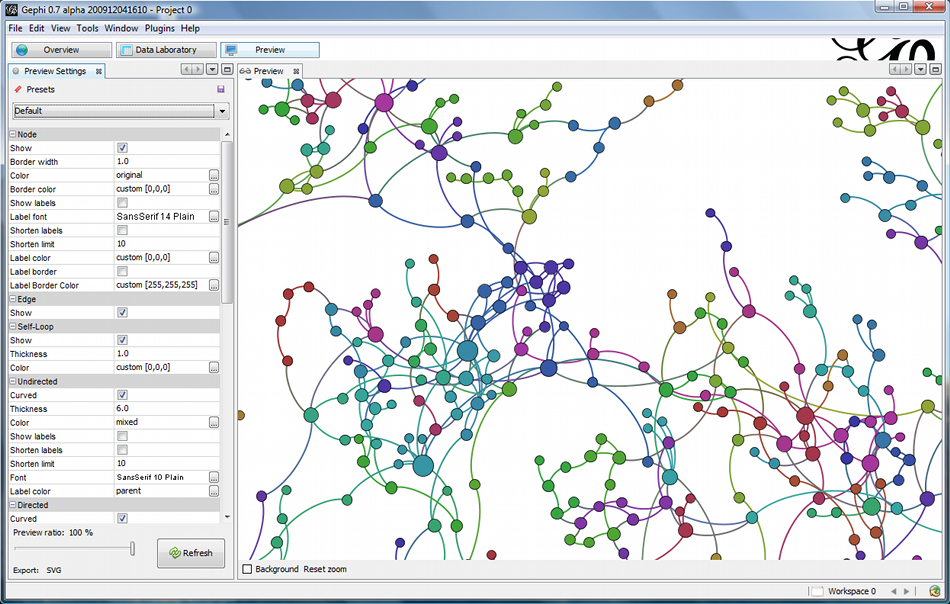
\includegraphics[width=.70\textwidth]{chapters/fig/gephiUm.png}
\caption{Captura de tela do software Gephi}
Fonte: gephi.github.io
\label{fig:gephiUm}
\end{figure}

\begin{figure}[htbp]
\centering
 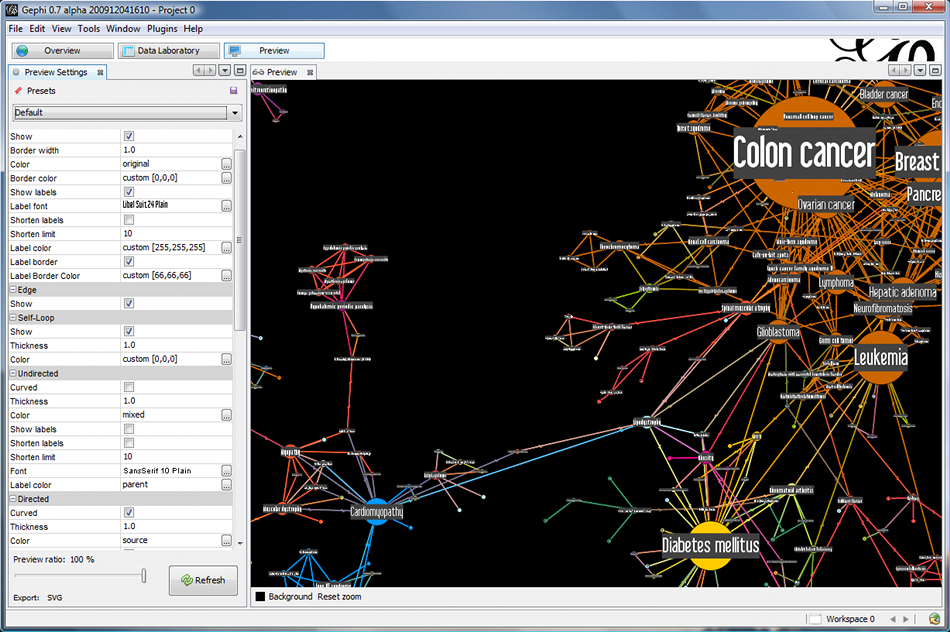
\includegraphics[width=.70\textwidth]{chapters/fig/gephiDois.png}
\caption{Captura de tela do software Gephi}
Fonte: gephi.github.io
\label{fig:gephiDois}
\end{figure}
\FloatBarrier

\pagebreak

\subsection{O modelo Dynagraph}
O modelo Dynagraph \cite{dynagraph} é baseado na primeira proposta em \cite{dynagraph2012}, que por sua vez é baseado no modelo
de \cite{kim}, porém o Dynagraph usa sequências temporais para vértices, arestas, características modificáveis dos vértices e arestas e
o relacionamento entre suas características. Com isso, é formado um grafo com as informações necessárias para qualquer instante no tempo.
O Dynagraph é capaz de visualizar o comportamento do grafo ao longo de um período de tempo, e editá-lo. A ferramenta construída permite
visualizar previsões e processos dinâmicos em vários contextos e realizar simulações preditivas sobre estes eventos \cite{dynagraph}.

Um grafo dinâmico é definido por $G^t$, que ocorre no intervalo $t = [t_s,t_f]$, onde $t_s$ é o tempo inicial e $t_f$ é o tempo final.
$G^t = (V^{t_v}, E^{t_e})$, onde $t_v \subseteq t$ e $t_e \subseteq t$, e $V^{t_v}$ e $E^{t_e}$ funções que geram vértices e arestas
respectivamente, em função do intervalo $t=t_v \cup t_e$.

As estruturas $V^{t_v} = \{O^{t_v}, F^{t_v}\}$ para vértices e $E^{t_e} = \{O^{t_e}, F^{t_e}\}$ para arestas são semelhantes,
onde $O^{t_v} = \{O_{0_v}, O_{1_v},..., O_{i_v}\}$ e $O^{t_e} = \{O_{0_e}, O_{1_e},..., O_{i_e}\}$ os objetos indexados de objetos,
e $F^{t_v} = \{F^{t_v}_{0_v}, F^{t_v}_{1_v},..., F^{t_v}_{w_v}\}$ e $F^{t_e} = \{F^{t_e}_{0_e}, F^{t_e}_{1_e},..., F^{t_e}_{w_e}\}$ os
conjuntos indexados de características modificáveis destes objetos \cite{dynagraph}.

A estrutura de dados usada no Dynagraph segue a Notação de Objeto Javascript (JSON), que é um formato de texto de intercâmbio de dados \cite{douglas}.
A figura \ref{fig:jsondyn} mostra como é essa estrutura seguindo três objetos principais: ``metadata'', ``binding'' e ``data''.

Em ``metadata'' são definidos os campos para utilização de qualquer identificador, por exemplo é possível utilizar ``ini'' e ``fim'' no
lugar de ``start'' e ``end'' respectivamente.

Em ``binding'' são definidas as características dos vértices e arestas. Seguindo o exemplo da figura \ref{fig:jsondyn}, ``vertex'' poderá
ser do tipo ``v1'', ``v2'' e ``v3'', onde cada tipo contém informações da forma do vértice. Essa forma pode ser uma imagem no formato
``png'' ou ``jpg'' ou customizada com as seguintes características:
\begin{itemize}
\item path: círculo ou seta;
\item fillColor: cor do preenchimento;
\item strokeColor: cor da borda;
\item fillOpacity: opacidade;
\item scale: tamanho;
\item strokeWeight: espessura da borda.
\end{itemize}
A aresta, ou ``polyline'', segue uma estrutura semelhante a do ``vertex'', porém com algumas particularidades como repetição de um símbolo
ao longo da aresta, e uma customização no campo ``path'' seguindo a notação
SVG\footnote{\label{note} Scalable Vector Graphics - é uma forma de descrever de forma vetorial desenhos e gráficos bidimensionais}.

Em ``data'' são definidos os elementos do grafo, os tempos de início e fim de cada elemento ou tempo de existência.
No caso dos vértices, a posição de cada elemento pode ser escrita no formato UTM ou latitude e longitude.
O tipo de cada elemento, descrito em ``binding'', e no caso das arestas, são definidos os pontos de origem e destino.

Na figura \ref{fig:jsondyn} vemos a estrutura de construção de um grafo dinâmico.
Os campos ``metadata'' e ``binding'' foram omitidos para evidenciar o objeto ``data''.
\FloatBarrier
\begin{center}
  \line(1,0){450}
\end{center}
\lstinputlisting[language=Java]{chapters/new.json}
\begin{figure}[htbp]
  \begin{center}
    \line(1,0){450}
  \end{center}
  \centering
  \caption{Estrutura JSON usada pelo Dynagraph}
  \label{fig:jsondyn}
\end{figure}

A figura \ref{fig:dynagraph} demonstra os dados do código da figura \ref{fig:jsondyn} sendo utilizados no software
Dynagraph com variações temporais no Grafo e nas características de seus Vértices e Arestas.

\FloatBarrier
\begin{figure}[htbp]
\centering
 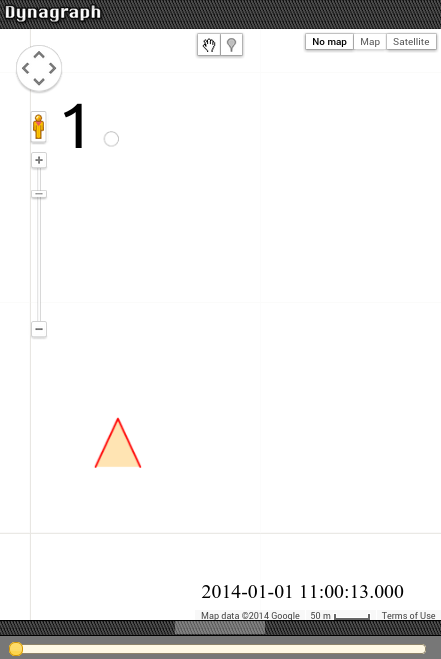
\includegraphics[width=.45\textwidth]{chapters/fig/b1mod.png}
 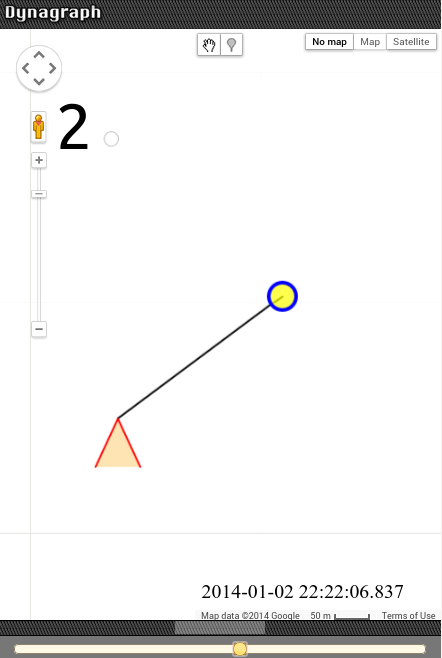
\includegraphics[width=.45\textwidth]{chapters/fig/b2mod.png}
 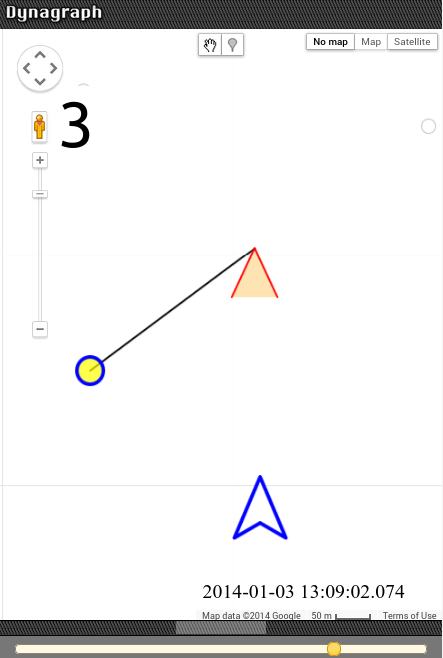
\includegraphics[width=.45\textwidth]{chapters/fig/b3mod.png}
 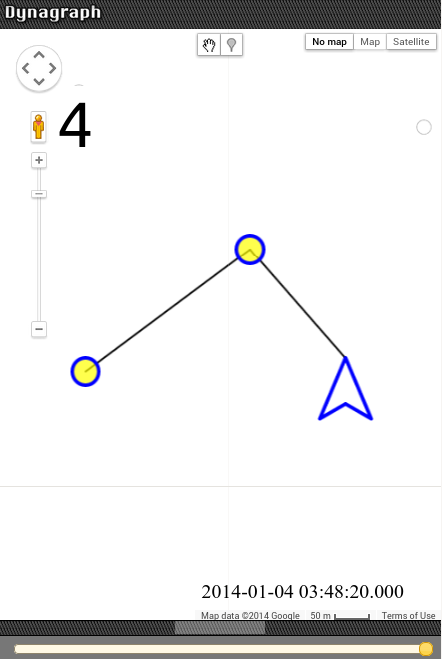
\includegraphics[width=.45\textwidth]{chapters/fig/b4mod.png}
\caption{Capturas de tela do software Dynagraph}
\label{fig:dynagraph}
\end{figure}

